% Number 811
% CAPMA Algebra Units 
% Clay/Jax chase - algebraic
% JG

% Watermark
\AddToShipoutPicture*{\BackgroundPic}

\addtocounter {ProbNum} {1}

%\begin{floatingfigure}[r]{.44\textwidth}
%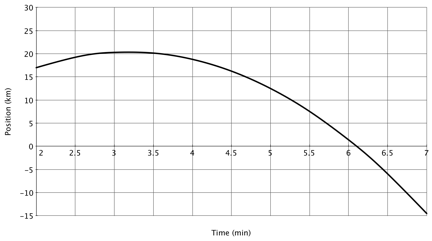
\includegraphics[scale=.5]{/Users/jgates/desktop/latex/pics/xgraph2}
%\end{floatingfigure}
 
{\bf \Large{\arabic{ProbNum}}} Jax is sitting by the side of the road on his motorcycle when Clay zips by at 30 meters per second.  Jax immediately takes off in pursuit, driving with a constant acceleration.  Jax accelerates to Clay's speed within 15 seconds. \bigskip

How far behind Clay will Jax be at that moment that their speeds are equal?  Use algebraic methods. \paragraph{}
\noindent

%\begin{center}
%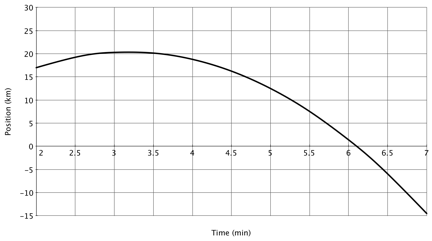
\includegraphics[scale=1]{/Users/jgates/desktop/latex/pics/xgraph2}
%\end{center}

\vfill
\newpage